\chapter{Una Breve Introducción a la Olimpiada}

¡Seas bievenido a la escena de la olimpiada! 
Si decides quedarte, el camino será una \dots, hmm, dura travesía, pero, 
aquí es donde encuentras las cosas más bellas que hay en la vida. 
Tanto un lema chino super potente y fumado como grandes amistades 
y experiencias inolvidables :)

No me creas a mi, pregúntenle a cualquier personas dentro de este proceso. 
Todos y cada uno de estos individuos te explicará de una forma 
muy linda como la olimpiada ha cambiado su vida 
y todo lo que han aprendido de ella. La Olimpiada de Matemáticas no 
es solamente matemáticas (y aunque lo fuera, seguiría siendo maravillosa), 
sino un mundo lleno de personitas apasionadas por una misma área, 
que se apoyan entre sí, se retan entre sí y se entienden los unos a los otros. 
Puede que hallas encontrado el mundo al que perteneces. 

Además, si resistes el suficiente tiempo, 
verás un montón de problemas geniales. 

\begin{figure}[h]
    \centering
    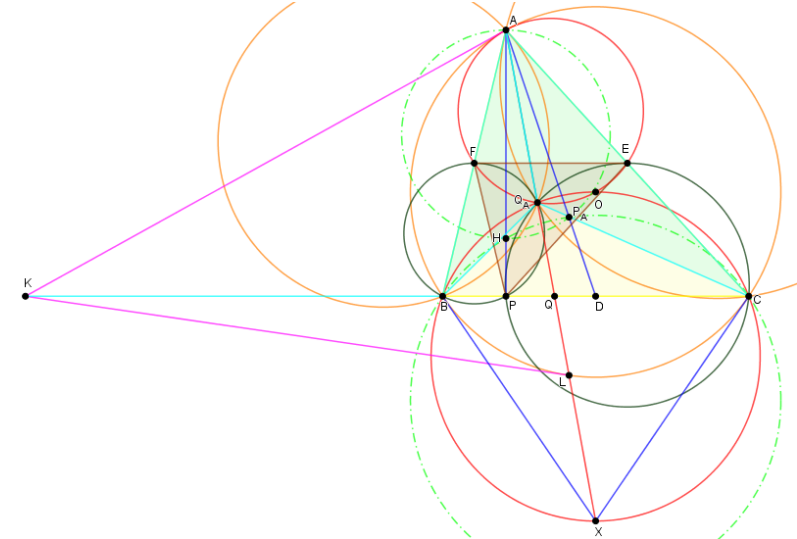
\includegraphics[height=9cm]{polymotiv.png} 
    \caption{Caracterizaciones del $A$-Humpty Point 
    y $A$-Dumpty Point del $\triangle ABC$}
\end{figure}

Este capítulo sería mil veces mejor si me dedicara a explicar 
todas esas caracterizaciones de Humpty y Dumpty pero ni modo; 
es lo que hay.

\section{Las Cuatro Áreas}

Es importante conocer unas cosillas sobre como se manejan las 
matemáticas en las olimpiadas, pues manejan solo cuatro áreas de las 
cientas que hay:

\begin{itemize}
    \ii Álgebra (alge pa los compas).
    \ii Combinatoria (combi pa los compas).
    \ii Geometría (geo pa los compas).
    \ii Teoría de Números (números pa los compas).
\end{itemize}

Cada una, será abordada en una parte distinta del libro. 
Es de suma importancia dominar todas, pues su presencia 
en las competencias es igual (además de que todas son sumamente bonitas). 
Es muy común que se cruzen entre sí, no se sorprendan cuando suceda.

\section{Sobre los Problemas de Olimpiada}

Me otorgaré el derecho de asumir dos cosas: primera, 
te gustan las matemáticas (seamos honesto, ¿a quién no?, son bellísimas);  
y segunda, quieres mejorar resolviendo problemas de matemáticas.

Partiendo de ahí, revisemos lo elemental.

La forma más sencilla de ver un problema de olimpiada de matemáticas 
es como un \textbf{puzzle}, es decir, un rompecabezas o un juego mental. 

A diferencia de lo que se ve en la escuela, 
aquí no se te da una fórmula que debes repetir mil veces en una lista 
con problemitas que tienen una mínima diferencia entre sí  
y nos es obvio el como se resuelve (en la mayoría de los casos; 
hay veces en las que el profe está de malas). Por supuesto que se 
trabajará con ejercicios, pues facilitan el entendimiento de conceptos 
además de que nos proporciona confianza, sin embargo, 
un ejercicio no es un problema de olimpiada. Un ejercicio sabemos como 
resolverlo casi inmediatamente; el que lo tengas bien o mal 
depende de que tan pulida tengas la técnica emplea el ejercicio. 
Por ejemplo, esto es un ejercicio:

\begin{example}
    Calcula $1234^5$ sin usar una calculadora. (SIN USAR CALCULADORA EH!!!!)
\end{example}

Al instante sabes como proceder, multiplica, CUIDADOSAMENTE, y ya :D.
Veamos el siguiente ejemplo:

\begin{example}
    Un chavo del inegi llega a una casa y le pregunta a la mujer dentro 
    cuantos niños tiene y cual es la edad de cada uno.

    "Tengo tres hijas, sus edades son números enteros y 
    el producto de sus edades es 36", dice la madre.

    "No es suficiente información", dice el compa.

    "Te diría la suma de sus edades, pero aun así seguirías confundido". 
    
    "Desearía que me dijera algo más".

    "Bueno, mi hija más grande, Marcela, no tiene amigos".

    ¿Cuáles son las edades de las tres hijas?
\end{example}

A primera vista, resolverlo parece imposible, 
!No hay suficiente información para determinar sus edades!
Por esa razon, ese es un problema, uno divertido por cierto 
(la respuesta está al final de el capítulo por si te atascas).

Un problema debe ser misterioso e interesante. Si no fuese misterioso, 
lo resolverías al verlo, y si no fuese interesante, ni siquiera lo 
intentarías en primer lugar. Si realmente cumple ambas expectativas, 
le dedicarás bastante tiempo y esfuerzo para hacerlo.

Si eres un inexperto en resolver problemas, seguramente te rendirás 
facilmente. Un veterano de la resolución de problemas al contrario, 
intentará confiadamente un montón de caminos al iniciar. Puede que no 
resuelva el problema, pero será un progreso. Y entonces, 
técnicas específicas entrarán en juego. Eventualmente, 
el problema estará resuelto. 

\begin{moral}
    Un experto opera de lo general a lo específico. 
\end{moral}

Primero intenta varias \textbf{estrategias}; en la que se vea progreso, 
le aplica \textbf{tácticas} que suelen repetirse en varios problemas 
de esa clase; y, finalmente en la táctica que funciona,  
le mete \textbf{mousekeherramientas 
misteriosas} que truenan el problema. Es claro, la dificultad del problema 
es un indicador de que tan extenso es este proceso, no obstante, hay 
que irnos preparando para las \textit{marranadas} que resolverán más adelante 
(quise decir, las \textit{bellezas} que resolverán más adelante).

Un problema demanda muchísima más reflexión y \textbf{creatividad}. 
Este último concepto es entrenable, 
pues al practicar muchísimo se va generando una \textit{intuición} 
de lo que funciona y lo que no en cierta situación.  

Les dejo un problema recreacional más antes de continuar. 
Se dice que Elon Musk le preguntaba esto a los aplicantes de Space X 
durante sus entrevistas.

\begin{problem}
    \jp
    Sales de tu casa, viajas una milla al sur, luego una al este, 
    y después una milla al norte. 
    ¡Al finalizar el recorrido regresaste a tu casa! ¿Donde vives?
\end{problem}

\subsection{Solución al Problema del Chavo del Inegi}

\begin{figure}[h]
    \centering
    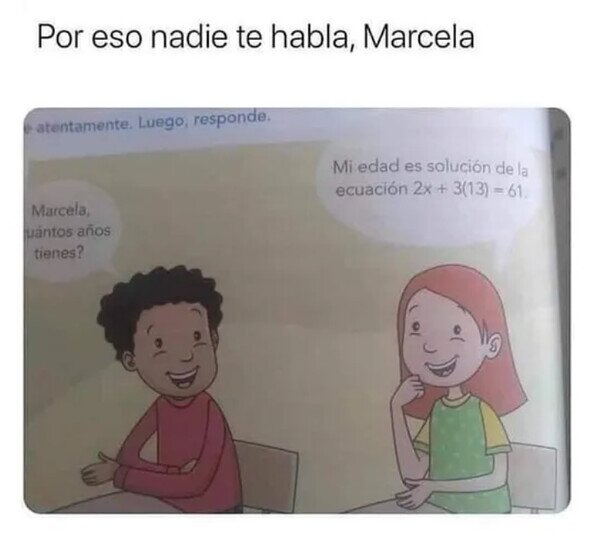
\includegraphics[height=8cm]{marcelasinamigos.jpg} 
    \caption{Te mereces todo lo malo que te pase, Marcela}
\end{figure}

Saliste igual que tu mamá, Marcela.

Volviendo al problema, 
estas son las ternas de enteros cuyo producto es 36 junto a su suma: 
$(1, 1, 36)$, que suma 38, $(1, 2, 18)$, que suma 21, 
$(1, 3, 12)$, que suma 16, $(1, 4, 9)$, que suma 14,
$(1, 6, 6)$, que suma 13, $(2, 2, 9)$, que suma 13,
$(2, 3, 6)$, que suma 11, $(3, 3, 4)$, que suma 10.
OHH! Ahora se ve que está sucediendo ¿no? 
Por la segunda declaración de la madre, sabemos que las edades son 
$(1, 6, 6)$ o $(2, 2, 9)$, porque en los demás casos, 
con la suma de sus edades sabríamos cuáles son. 
Y por la tercera declaración, sabemos que hay una hermana mayor, eliminando la terna $(1, 6, 6)$ así que sabemos que 
las hijas tienen $2$, $2$ y $9$ años.
